\documentclass[xetex,mathserif,serif]{beamer}
\usepackage{polyglossia}
\setdefaultlanguage[babelshorthands=true]{russian}
\usepackage{minted}
\usepackage{tabu}

\useoutertheme{infolines}

\usepackage{fontspec}
\setmainfont{FreeSans}
\newfontfamily{\russianfonttt}{FreeSans}

\definecolor{links}{HTML}{2A1B81}
\hypersetup{colorlinks,linkcolor=,urlcolor=links}

\tabulinesep=0.7mm

\title{Пример архитектуры --- Bash}
\author[Юрий Литвинов]{Юрий Литвинов \newline \textcolor{gray}{\small\texttt{yurii.litvinov@gmail.com}}}

\date{19.02.2020г}

\begin{document}
	
	\frame{\titlepage}

	\section{Юнит-тестирование}

	\begin{frame}
		\frametitle{Сначала, внезапно, юнит-тесты}
		\begin{itemize}
			\item Любая программа содержит ошибки
			\item Если программа не содержит ошибок, их содержит алгоритм, который реализует эта программа
			\item Если ни программа, ни алгоритм ошибок не содержат, такая программа даром никому не нужна
		\end{itemize}
		Тестирование не позволяет доказать отсутствие ошибок, оно позволяет лишь найти ошибки, которые в программе присутствуют
	\end{frame}

	\begin{frame}
		\frametitle{Модульное тестирование}
		\begin{itemize}
			\item Тест на каждый отдельный метод, функцию, иногда класс
			\item Пишутся программистами
			\item Запускаются часто (как минимум, после каждого коммита)
			\item Должны всегда проходить
			\item Помогают быстро искать ошибки (вы ещё помните, что исправляли), рефакторить код (``ремни безопасности''), продумывать архитектуру (мешанину невозможно оттестировать), документировать код (каждый тест -- это рабочий пример вызова)
		\end{itemize}
	\end{frame}

	\begin{frame}
		\frametitle{Пример, JUnit 5}
		\begin{itemize}
			\item JUnit --- самая известная библиотека юнит-тестирования для Java
			\item JUnit 5 --- его последняя версия (часто до сих пор используется JUnit 4)
			\item Отлично интегрируется с IDEA
			\begin{itemize}
				\item Генерация заглушек тестов, запуск тестов прямо из редактора и т.д.
			\end{itemize}
			\item Тест --- это отдельный класс, в котором есть методы, помеченные аннотацией \mintinline{java}|@Test|
			\item Внутри теста обычно три фазы
			\begin{itemize}
				\item Настройка тестового окружения
				\item Выполнение действия, которое хотим тестировать
				\item Проверка результатов
				\begin{itemize}
					\item Вызовы assertEquals, assertNull, assertTrue и т.д.
				\end{itemize}
			\end{itemize}
		\end{itemize}
	\end{frame}

	\begin{frame}[fragile]
		\frametitle{Пример}
		\begin{small}
			\begin{minted}{java}
class StackTest {

    private Stack<Integer> stack;

    @BeforeEach
    void init() {
        stack = new Stack<>();
    }

    @Test
    void testSimpleCaseWithPushAndPop() {
        stack.push(1);
        var result = stack.pop();
        assertEquals(1, result);
        assertThrows(IllegalStateException.class, () -> stack.pop());
    }
}
			\end{minted}
		\end{small}
	\end{frame}

	\begin{frame}
		\frametitle{Ещё хорошие библиотеки}
		\begin{itemize}
			\item Apache Hamcrest --- библиотека матчеров
			\item NUnit, XUnit, Microsoft Unit Testing Framework --- для .NET
			\item Google Testing and Mocking Framework, CxxTest, Boost.Test, Catch, тысячи их для C++
			\item HUnit, HSpec, QuickCheck для Haskell
			\item FsUnit, FsCheck для F\#
			\item А ещё есть mock-объекты: Mockito, NSubstitute, ...
		\end{itemize}
	\end{frame}

	\begin{frame}
		\frametitle{Best practices}
		\begin{itemize}
			\item Независимость тестов
			\begin{itemize}
				\item Желательно, чтобы поломка одного куска функциональности ломала один тест
			\end{itemize}
			\item Тесты должны работать быстро
			\begin{itemize}
				\item И запускаться после каждой сборки
				\begin{itemize}
					\item Continuous Integration
				\end{itemize}
			\end{itemize}
			\item Тестов должно быть много
			\begin{itemize}
				\item Следите за Code coverage, должно быть близко к 100\%
			\end{itemize}
			\item Каждый тест должен проверять конкретный тестовый сценарий
			\begin{itemize}
				\item Нельзя ловить исключения в тесте без крайней нужды
				\item С большой осторожностью пользоваться Random-ом
			\end{itemize}
			\item Именование тестов: \url{http://stackoverflow.com/questions/155436/unit-test-naming-best-practices}
			\item Test-driven development
		\end{itemize}
	\end{frame}

	\section{Enterprise Fizz-Buzz}

	\begin{frame}
		\frametitle{Enterprise Fizz-Buzz}
		Задача:

		Для чисел от 1 до 100:
		\begin{itemize}
			\item если число делится на 3, вывести ``Fizz''
			\item если число делится на 5, вывести ``Buzz''
			\item если число делится и на 3, и на 5, вывести ``FizzBuzz''
			\item во всех остальных случаях вывести само число
		\end{itemize}

		Решение:

		\url{https://github.com/EnterpriseQualityCoding/FizzBuzzEnterpriseEdition}
	\end{frame}

	\begin{frame}
		\frametitle{Структура системы}
		\begin{center}
			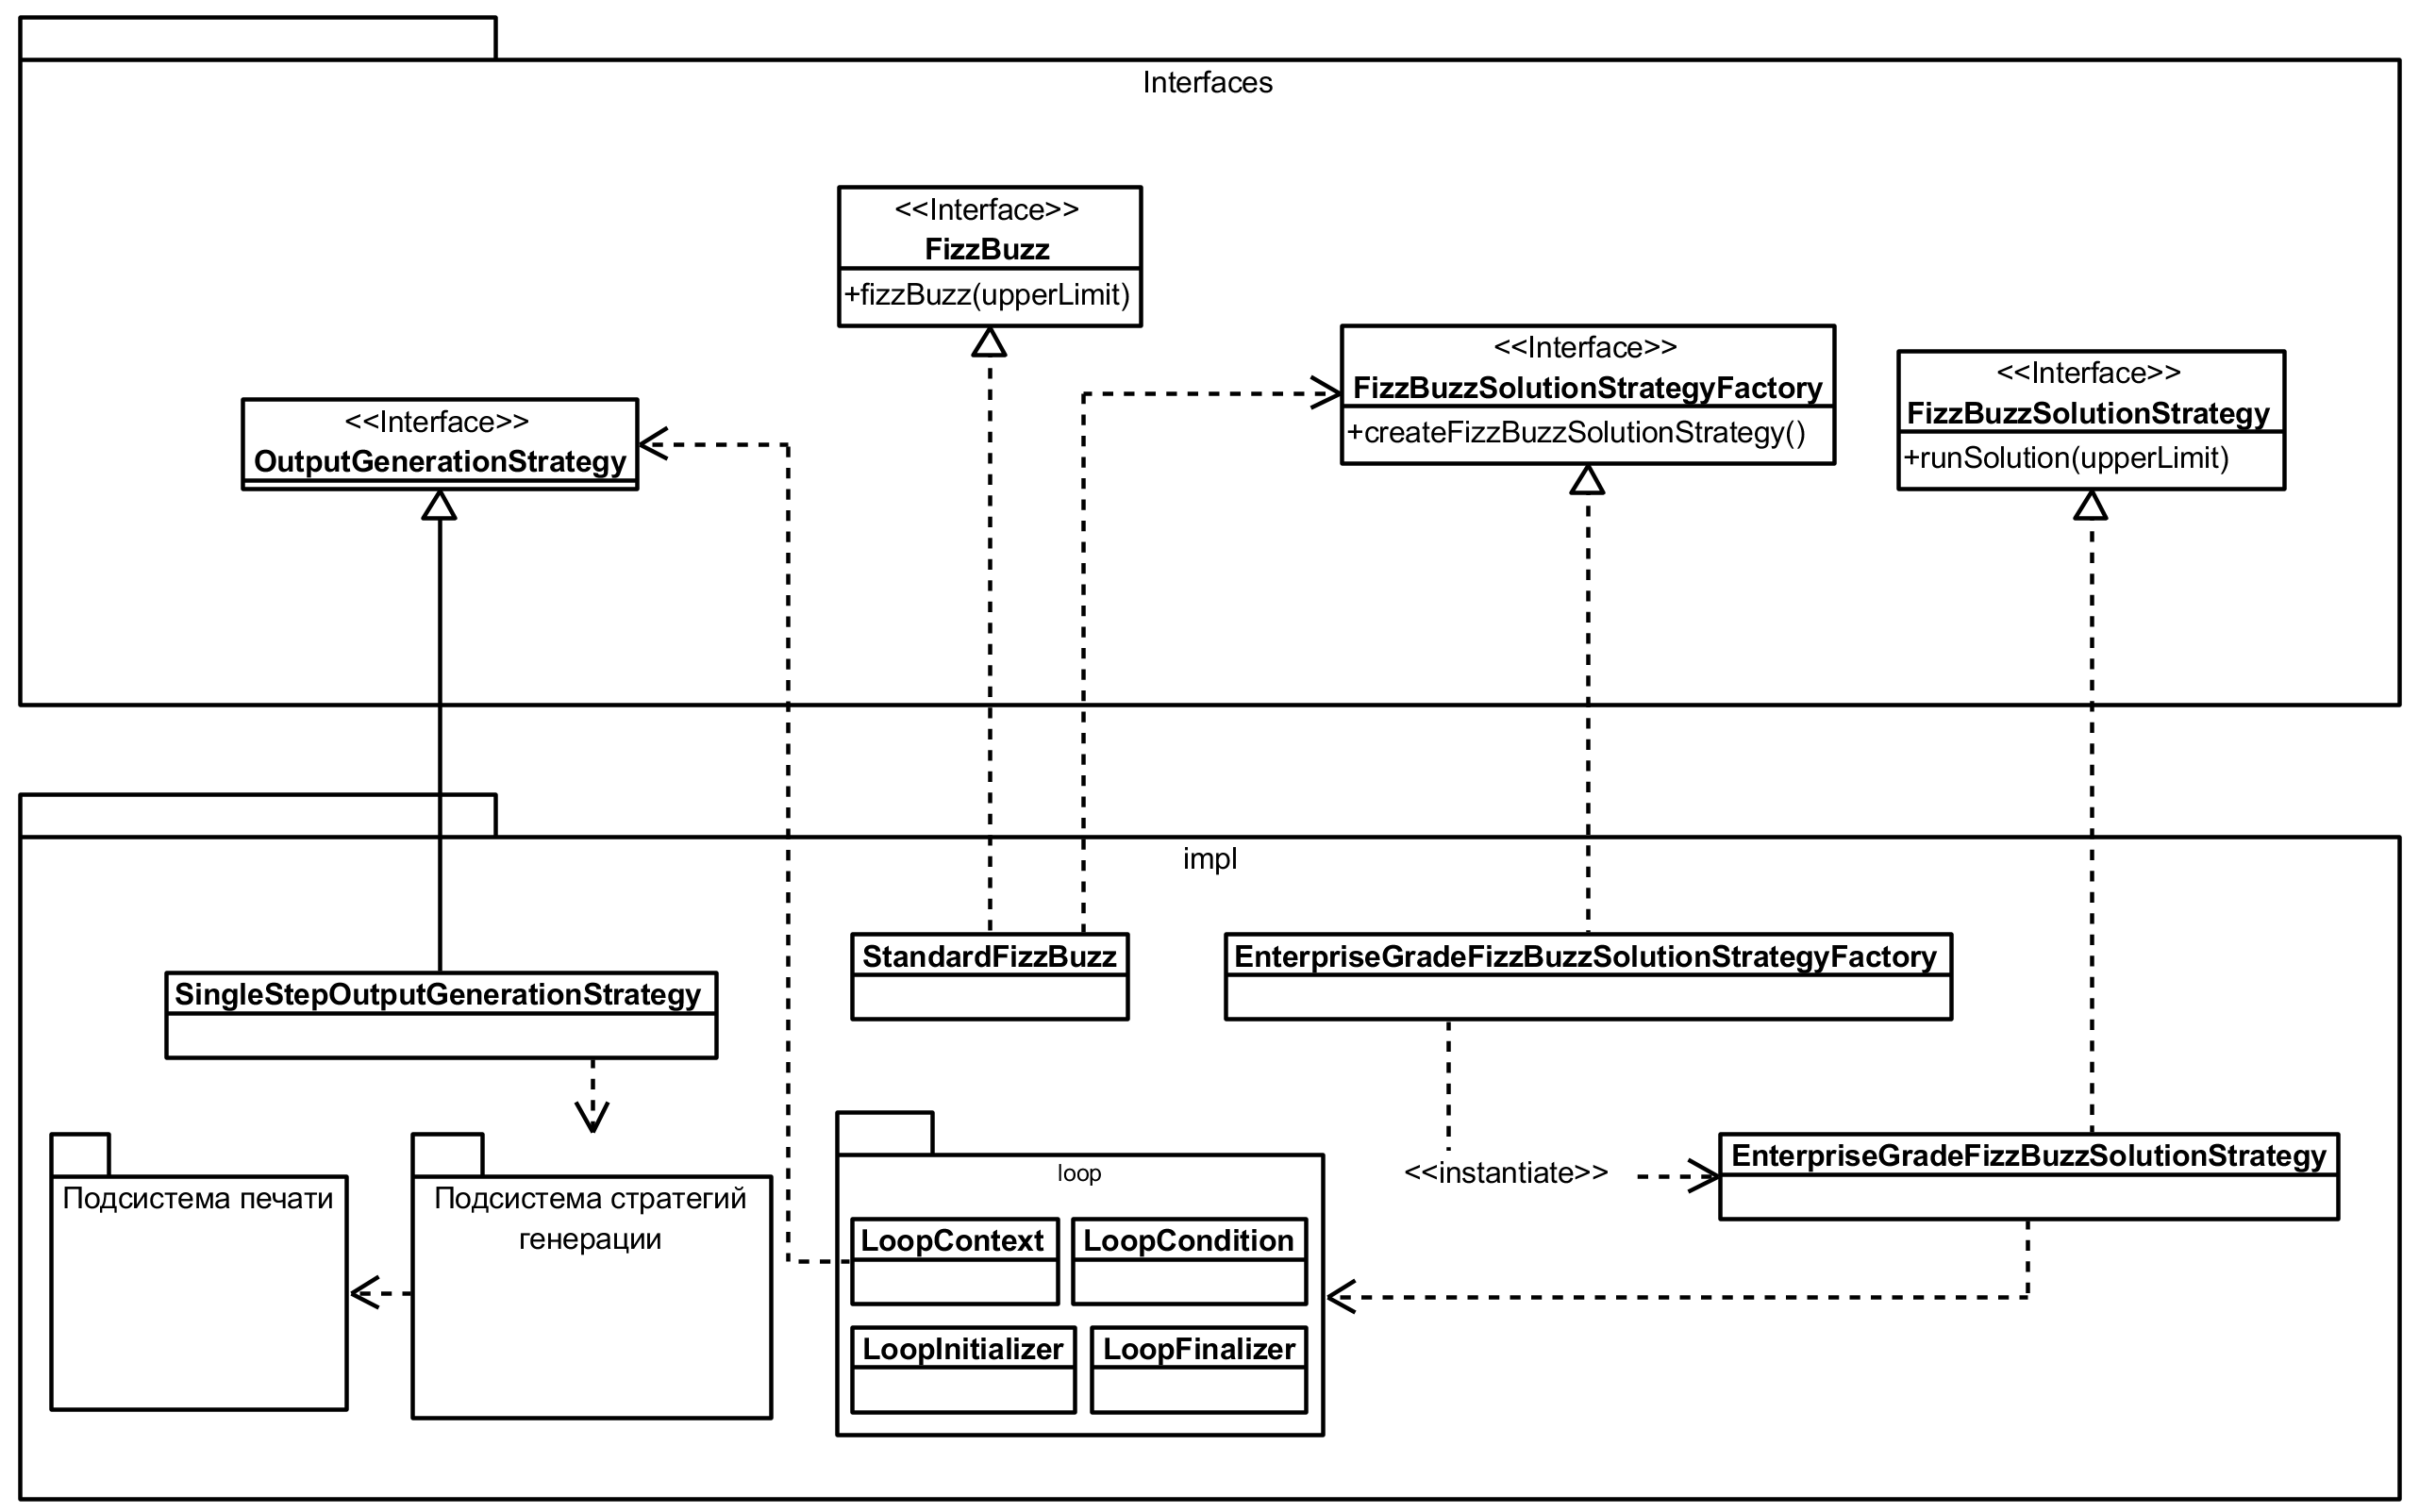
\includegraphics[width=\textwidth]{fizzBuzzArchitecture.png}
		\end{center}
	\end{frame}

	\begin{frame}
		\frametitle{Хорошие идеи}
		\begin{itemize}
			\item Separation of Concerns
			\item Dependency Inversion
			\item Dependency Injection
			\begin{itemize}
				\item Spring Framework
			\end{itemize}
			\item Паттерны ``Фабрика'', ``Стратегия'', ``Посетитель'', ``Адаптер'', что-то вроде паттернов ``Спецификация'' и ``Цепочка ответственности''
		\end{itemize}
	\end{frame}

	\begin{frame}
		\frametitle{Плохие идеи}
		\begin{itemize}
			\item Не выполняется принцип Keep It Simple Stupid
			\begin{itemize}
				\item Неправильно говорить ``строк кода написано'', правильно --- ``строк кода израсходовано''
			\end{itemize}
			\item ``Синтаксическое'' разделение на пакеты, а не ``семантическое''
			\begin{itemize}
				\item Отсуствие модульности, антипаттерн ``Big Ball of Mud''
			\end{itemize}
			\item Хардкод основных параметров вычисления
			\item Нет юнит-тестов, только интеграционные; нет логирования
			\item 1662 строки кода, очень мало комментариев (несмотря на недавно принятый пуллреквест ``Serious Documentation'')
			\begin{itemize}
				\item Отсутствие архитектурного описания
			\end{itemize}
		\end{itemize}
	\end{frame}

	\section{Bash}

	\begin{frame}
		\frametitle{Bash}
		\begin{itemize}
			\item Примерно 70К строк кода
			\item Исходный автор --- Brian Fox, maintainer --- Chet Ramey
			\item Первый релиз --- 1989
			\item Написан на C
			\item Архитектурное описание --- глава в \textit{The Architecture of Open Source Applications}, написанная Chet Ramey
		\end{itemize}
	\end{frame}

	\begin{frame}
		\frametitle{Архитектура Bash}
		\begin{center}
			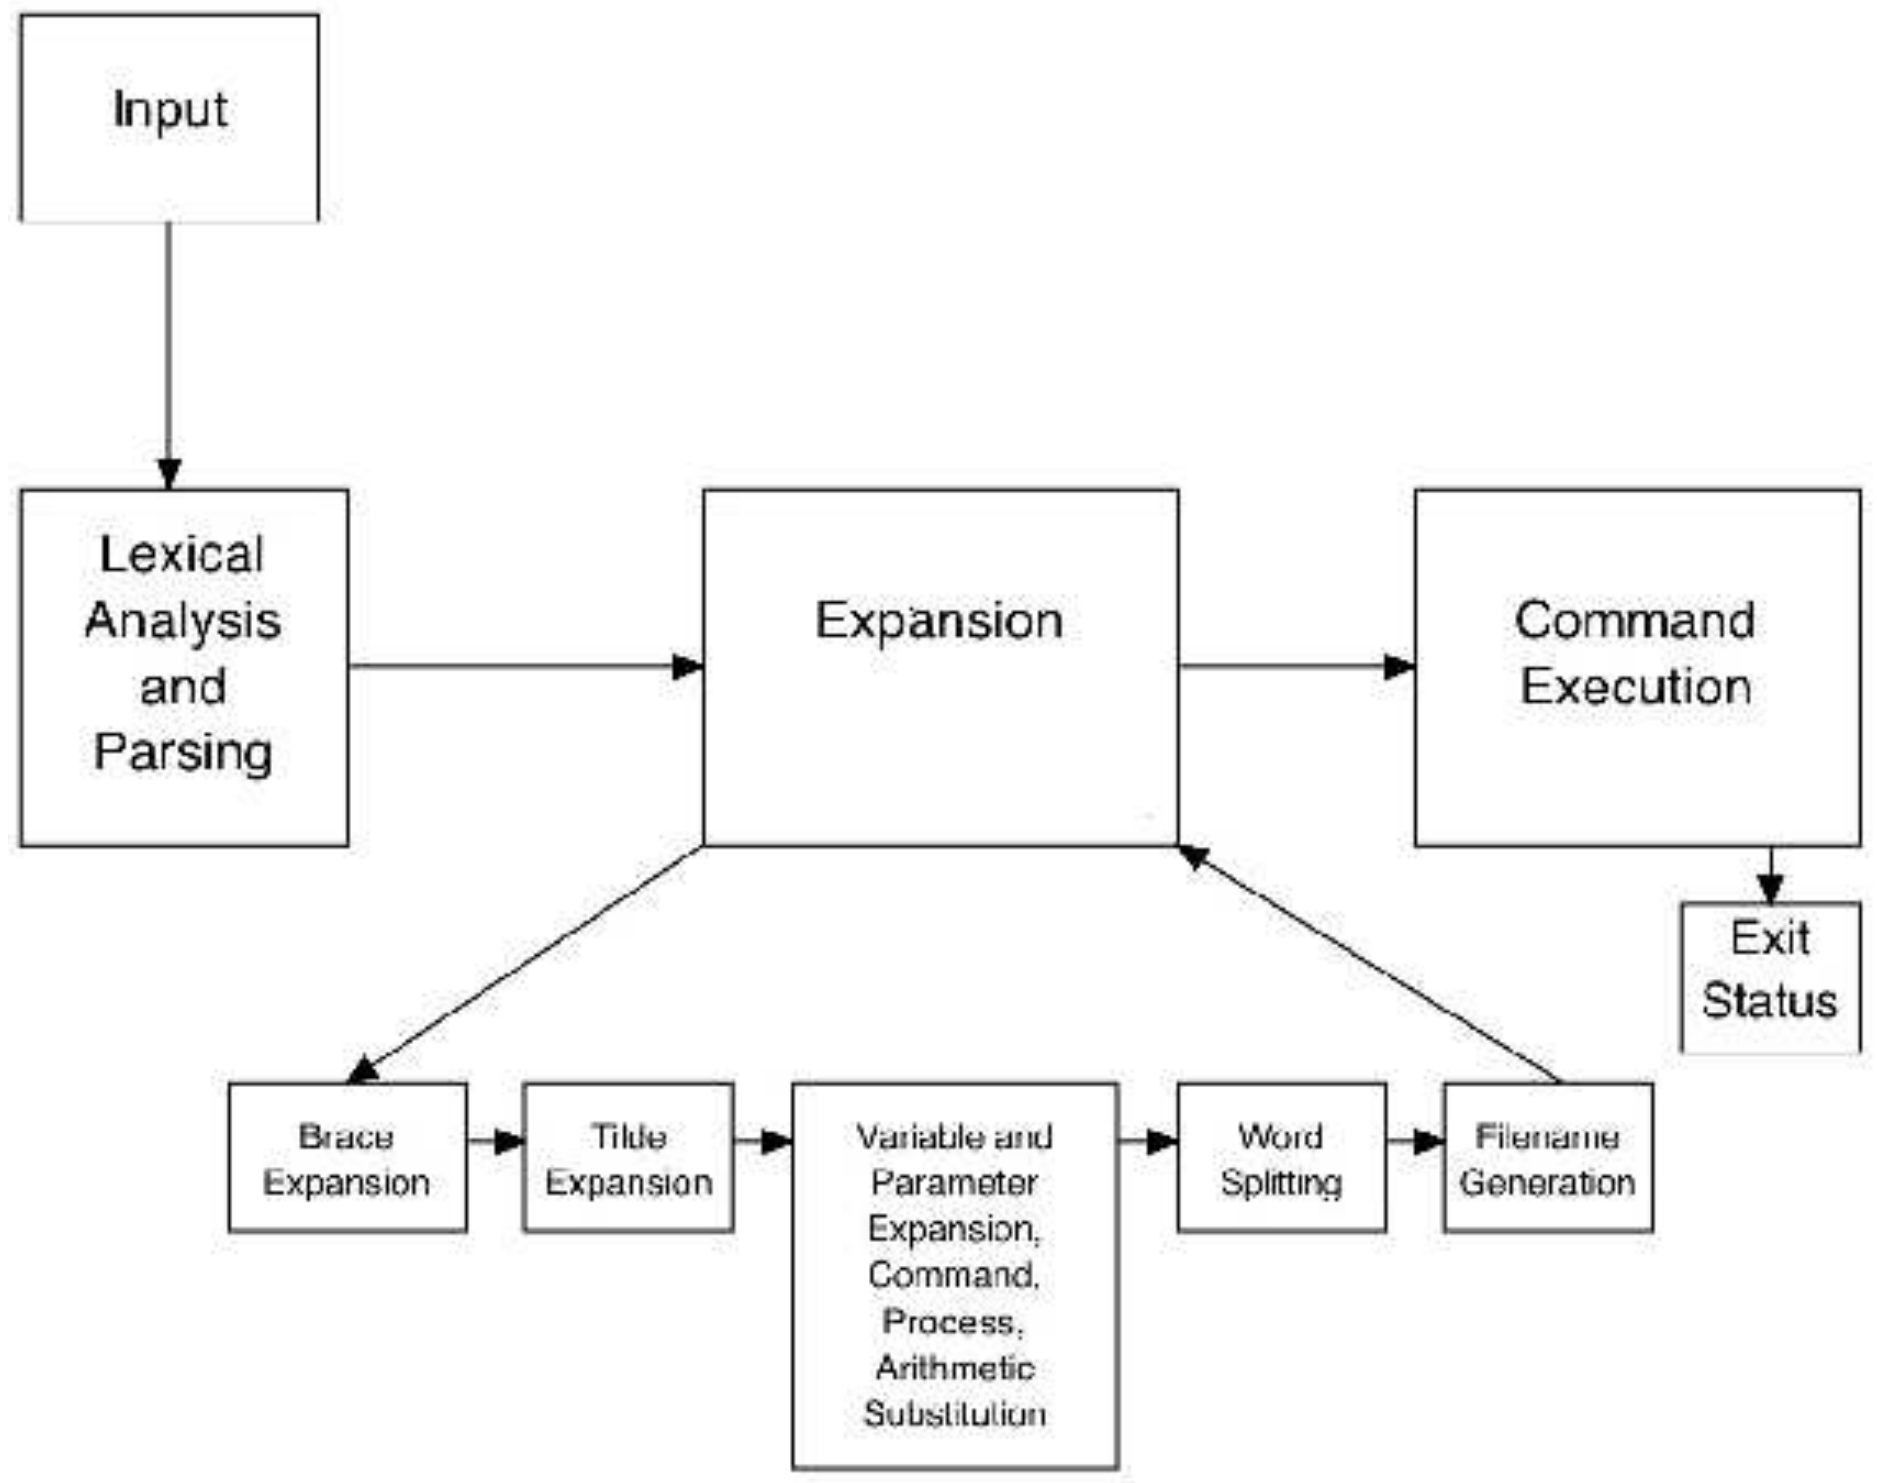
\includegraphics[width=0.7\textwidth]{bashArchitecture.png}
		\end{center}
	\end{frame}

	\begin{frame}[fragile]
		\frametitle{Основные структуры данных}
		\begin{minted}{c}
typedef struct word_desc {
    char *word; /* Zero terminated string. */
    int flags; /* Flags associated with this word. */
} WORD_DESC;
		\end{minted}

		\vspace{3mm}

		\begin{minted}{c}
typedef struct word_list {
    struct word_list *next;
    WORD_DESC *word;
} WORD_LIST;
		\end{minted}
	\end{frame}

	\begin{frame}
		\frametitle{Ввод с консоли}
		\begin{itemize}
			\item Библиотека Readline
			\begin{itemize}
				\item независимая библиотека, но пишется в основном для Bash
			\end{itemize}
			\item Цикл read/dispatch/execute/redisplay
			\item Dispatch table (или Keymap)
			\item Буфер редактирования, хитрый механизм расчёта действий для отображения
			\item Хранит все данные как 8-битные символы, но знает про Unicode
		\end{itemize}
	\end{frame}

	\begin{frame}[fragile]
		\frametitle{Синтаксический разбор}
		\begin{itemize}
			\item Зависимый от контекста лексический анализ
				\begin{minted}{sh}
for for in for; do for=for; done; echo $for
				\end{minted}
			\item Использует lex + bison
			\item Подстановка alias-ов выполняется лексером
			\item Сохранение и восстановление состояния парсера
		\end{itemize}
	\end{frame}

	\begin{frame}[fragile]
		\frametitle{Подстановки}
		\begin{minted}{sh}
${parameter:-word}
		\end{minted}

раскрывается в \textit{parameter}, если он установлен, и в \textit{word}, если нет

		\begin{minted}{sh}
pre{one,two,three}post
		\end{minted}

раскрывается в 

		\begin{minted}{sh}
preonepost pretwopost prethreepost
		\end{minted}

		Ещё бывает подстановка тильды и арифметическая подстановка, сопоставление шаблона
	\end{frame}

	\begin{frame}[fragile]
		\frametitle{Исполнение команд}
		\begin{itemize}
			\item Встроенные и внешние команды, обрабатываются единообразно
			\item Перенаправление ввода-вывода, отмена перенаправления
			\item Принимают набор слов
			\begin{itemize}
				\item Иногда обрабатывают по-особому, например, присваивание в \textit{export}
			\end{itemize}
			\item Присваивание --- тоже команда, но особая
			\item Перед запуском внешней команды --- поиск в PATH, кеширование результатов
			\item Job control, foreground и background
		\end{itemize}
	\end{frame}

	\begin{frame}[fragile]
		\frametitle{Lessons Learned}
		\begin{itemize}
			\item Комментарии к коммитам со ссылками на багрепорты с шагами воспроизведения
			\item Хороший набор тестов, в Bash их тысячи
			\item Стандарты, как внешние на функциональность шелла, так и на код
			\item Пользовательская документация
			\item Переиспользование
		\end{itemize}
	\end{frame}

	\section{Bash, на самом деле}

	\begin{frame}
		\frametitle{Архитектура Bash, на самом деле}
		\begin{itemize}
			\item J. Garcia et al., \textit{Obtaining Ground-Truth Software Architectures}
			\item 1 аспирант, 80 часов работы
			\item Верификация от Chet Ramey
			\item 70К строк кода, 200 файлов, 25 компонент
			\begin{itemize}
				\item 16 --- ядро, 9 --- утилиты
			\end{itemize}
			\item Структура папок почти не соответствует выделенным компонентам
		\end{itemize}
	\end{frame}

	\begin{frame}
		\frametitle{Архитектура Bash, на самом деле}
		\begin{center}
			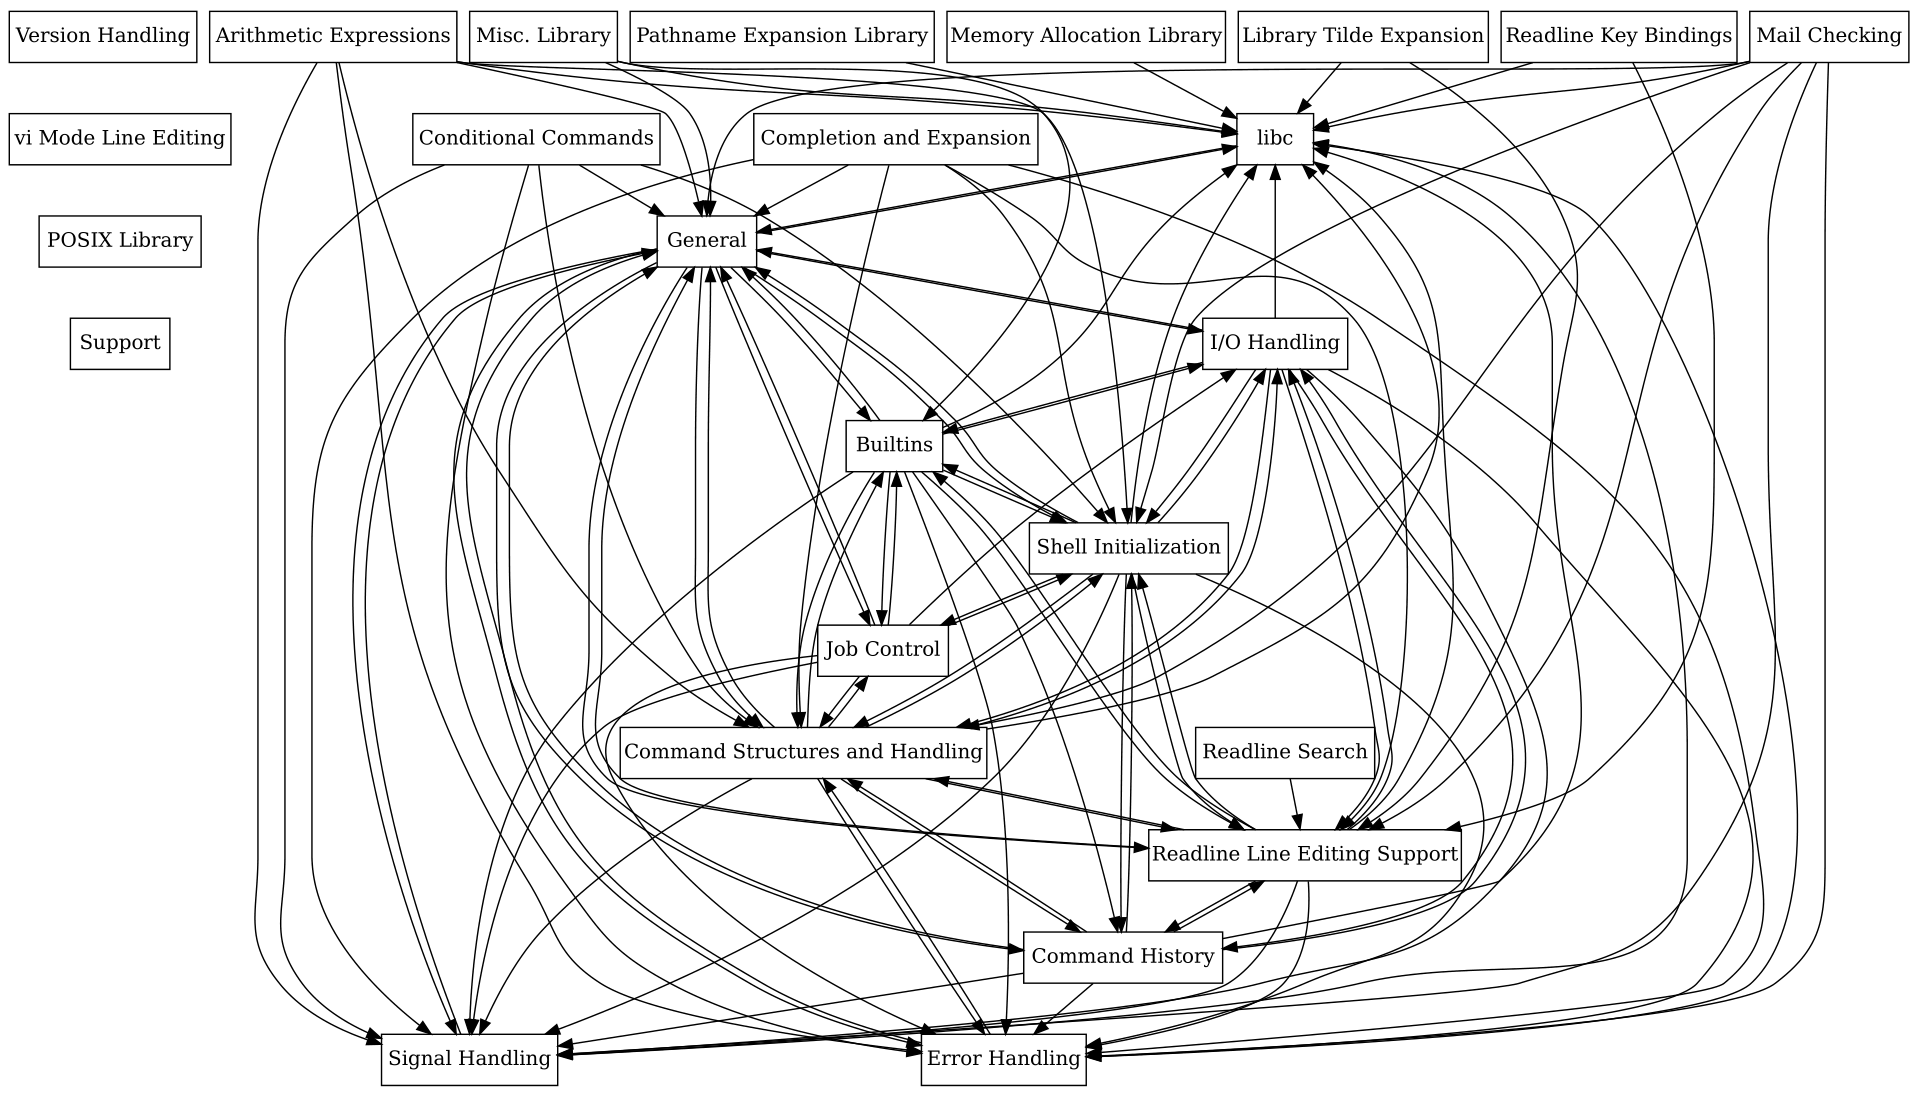
\includegraphics[width=\textwidth]{bashRealArchitecture.png}
		\end{center}
	\end{frame}

	\begin{frame}
		\frametitle{Результаты анализа кода}
		\begin{center}
			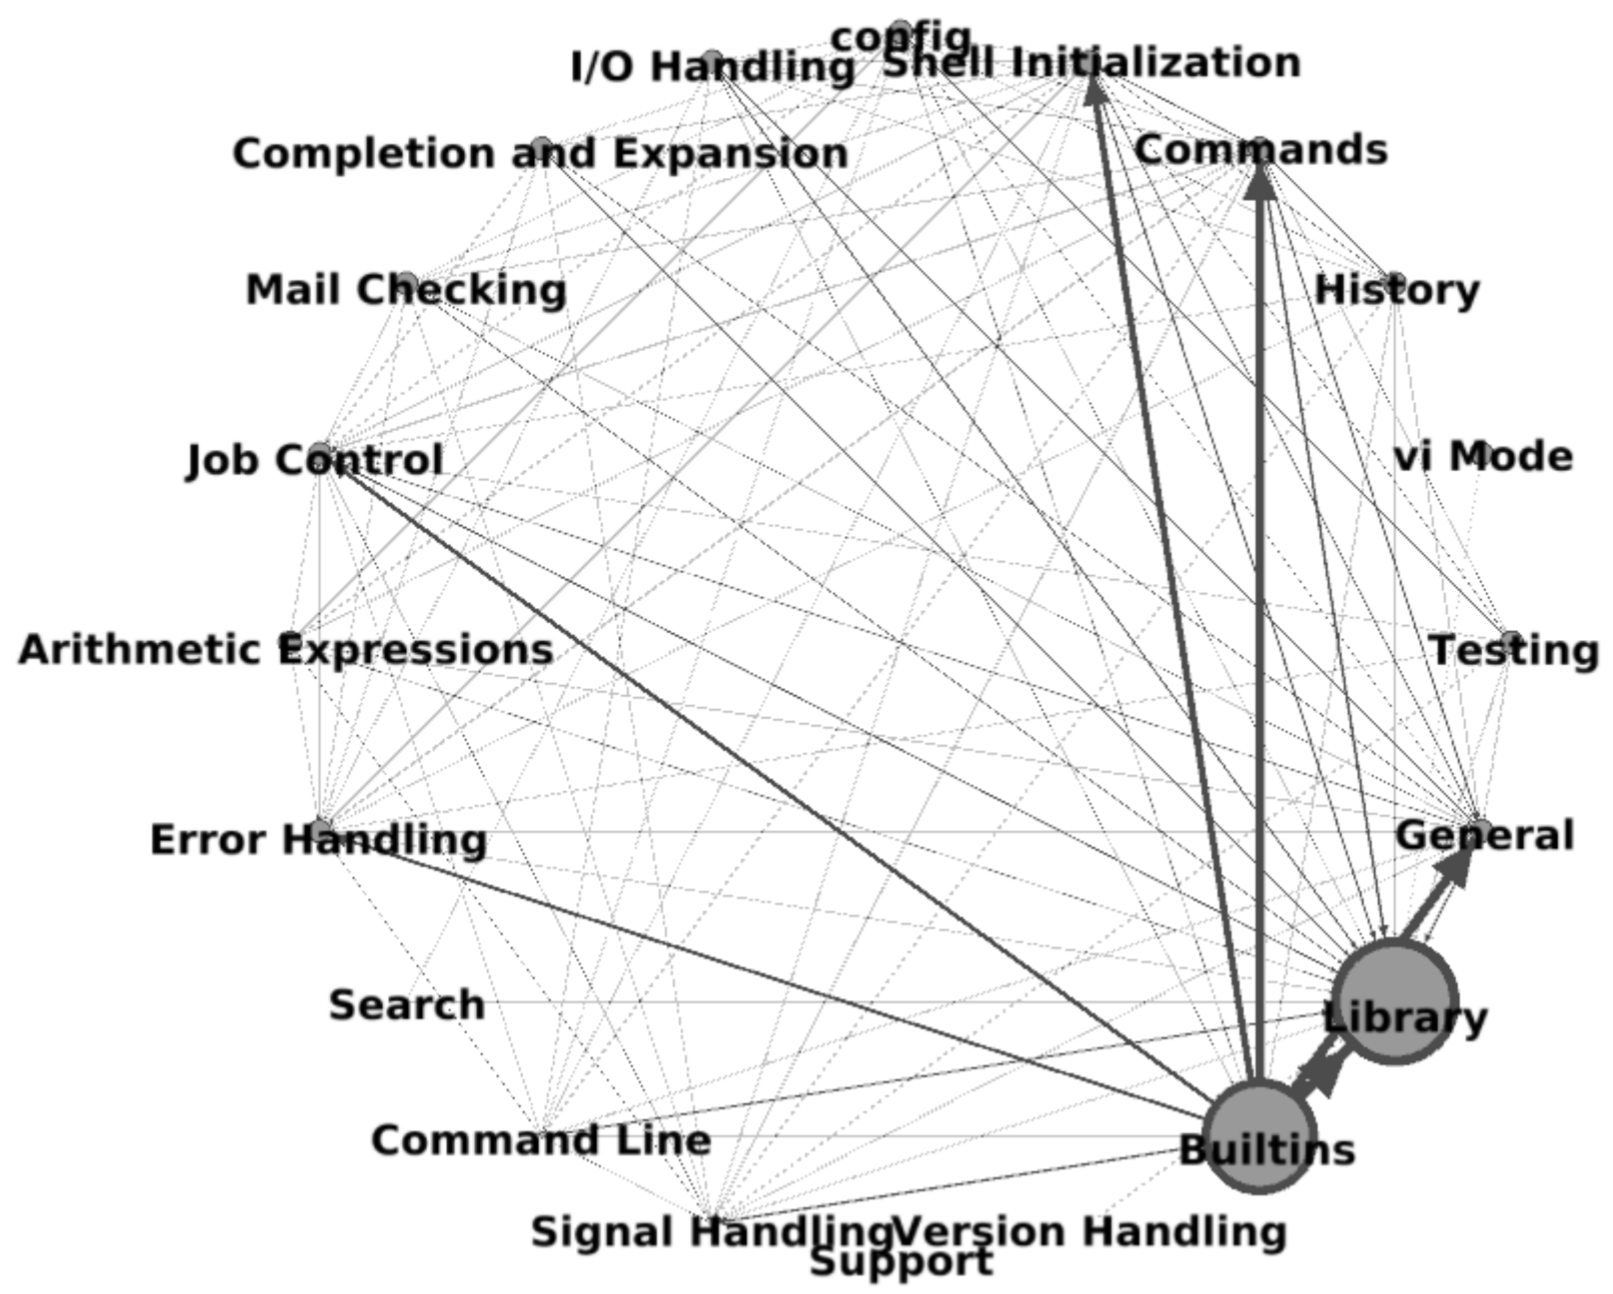
\includegraphics[width=0.7\textwidth]{bashAutomaticRecoveryArchitecture.png}
		\end{center}
	\end{frame}

	\begin{frame}
		\frametitle{Сравним с исходной}
		\begin{center}
			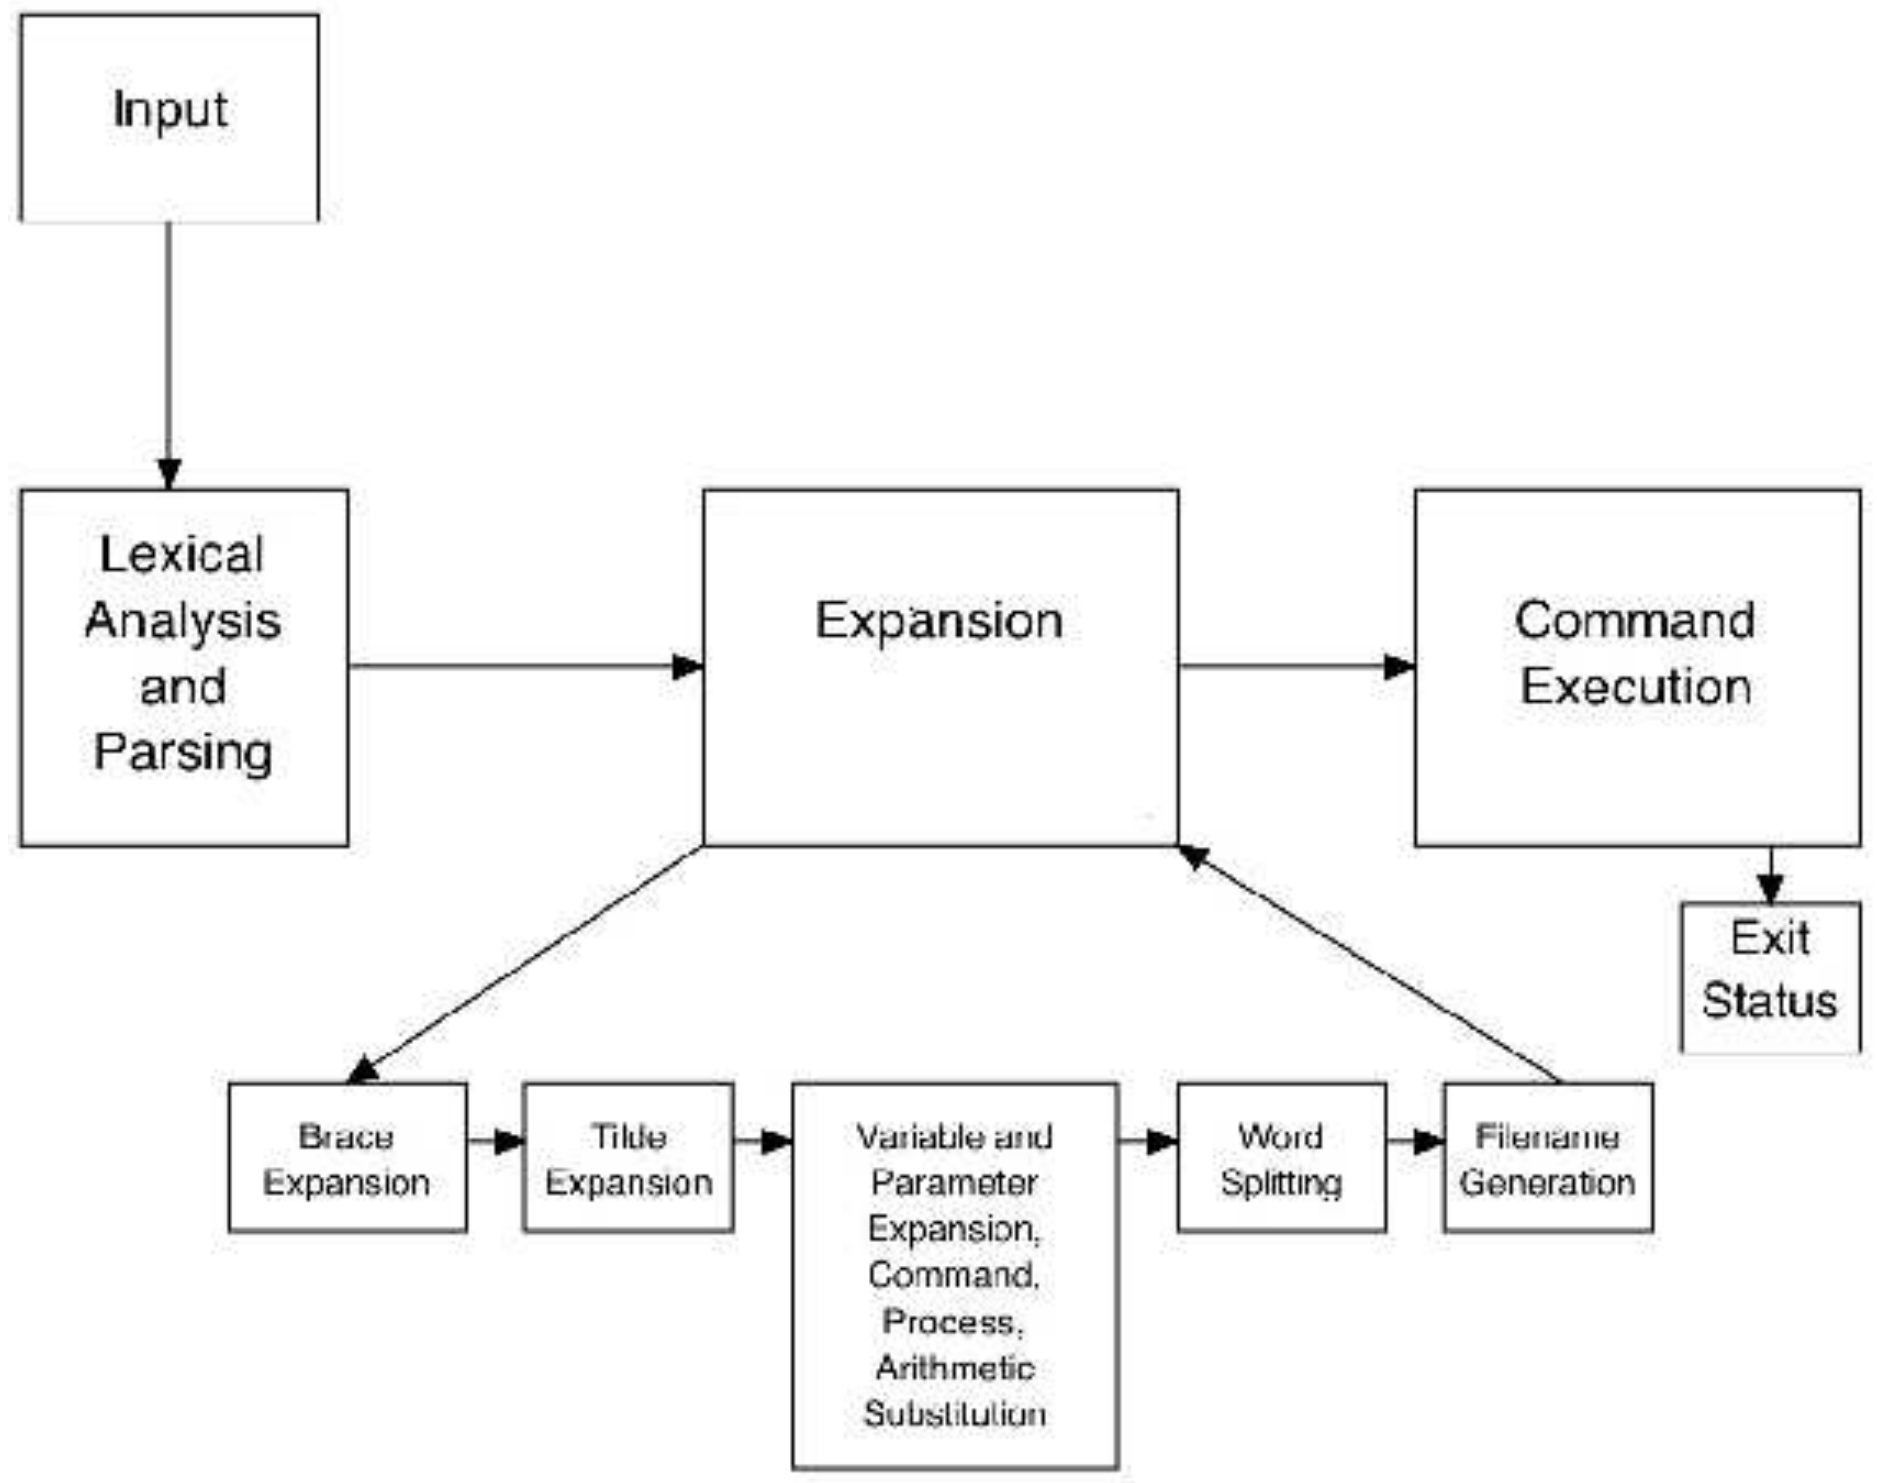
\includegraphics[width=0.7\textwidth]{bashArchitecture.png}
		\end{center}
	\end{frame}

	\begin{frame}
		\frametitle{Job Control}
		\begin{center}
			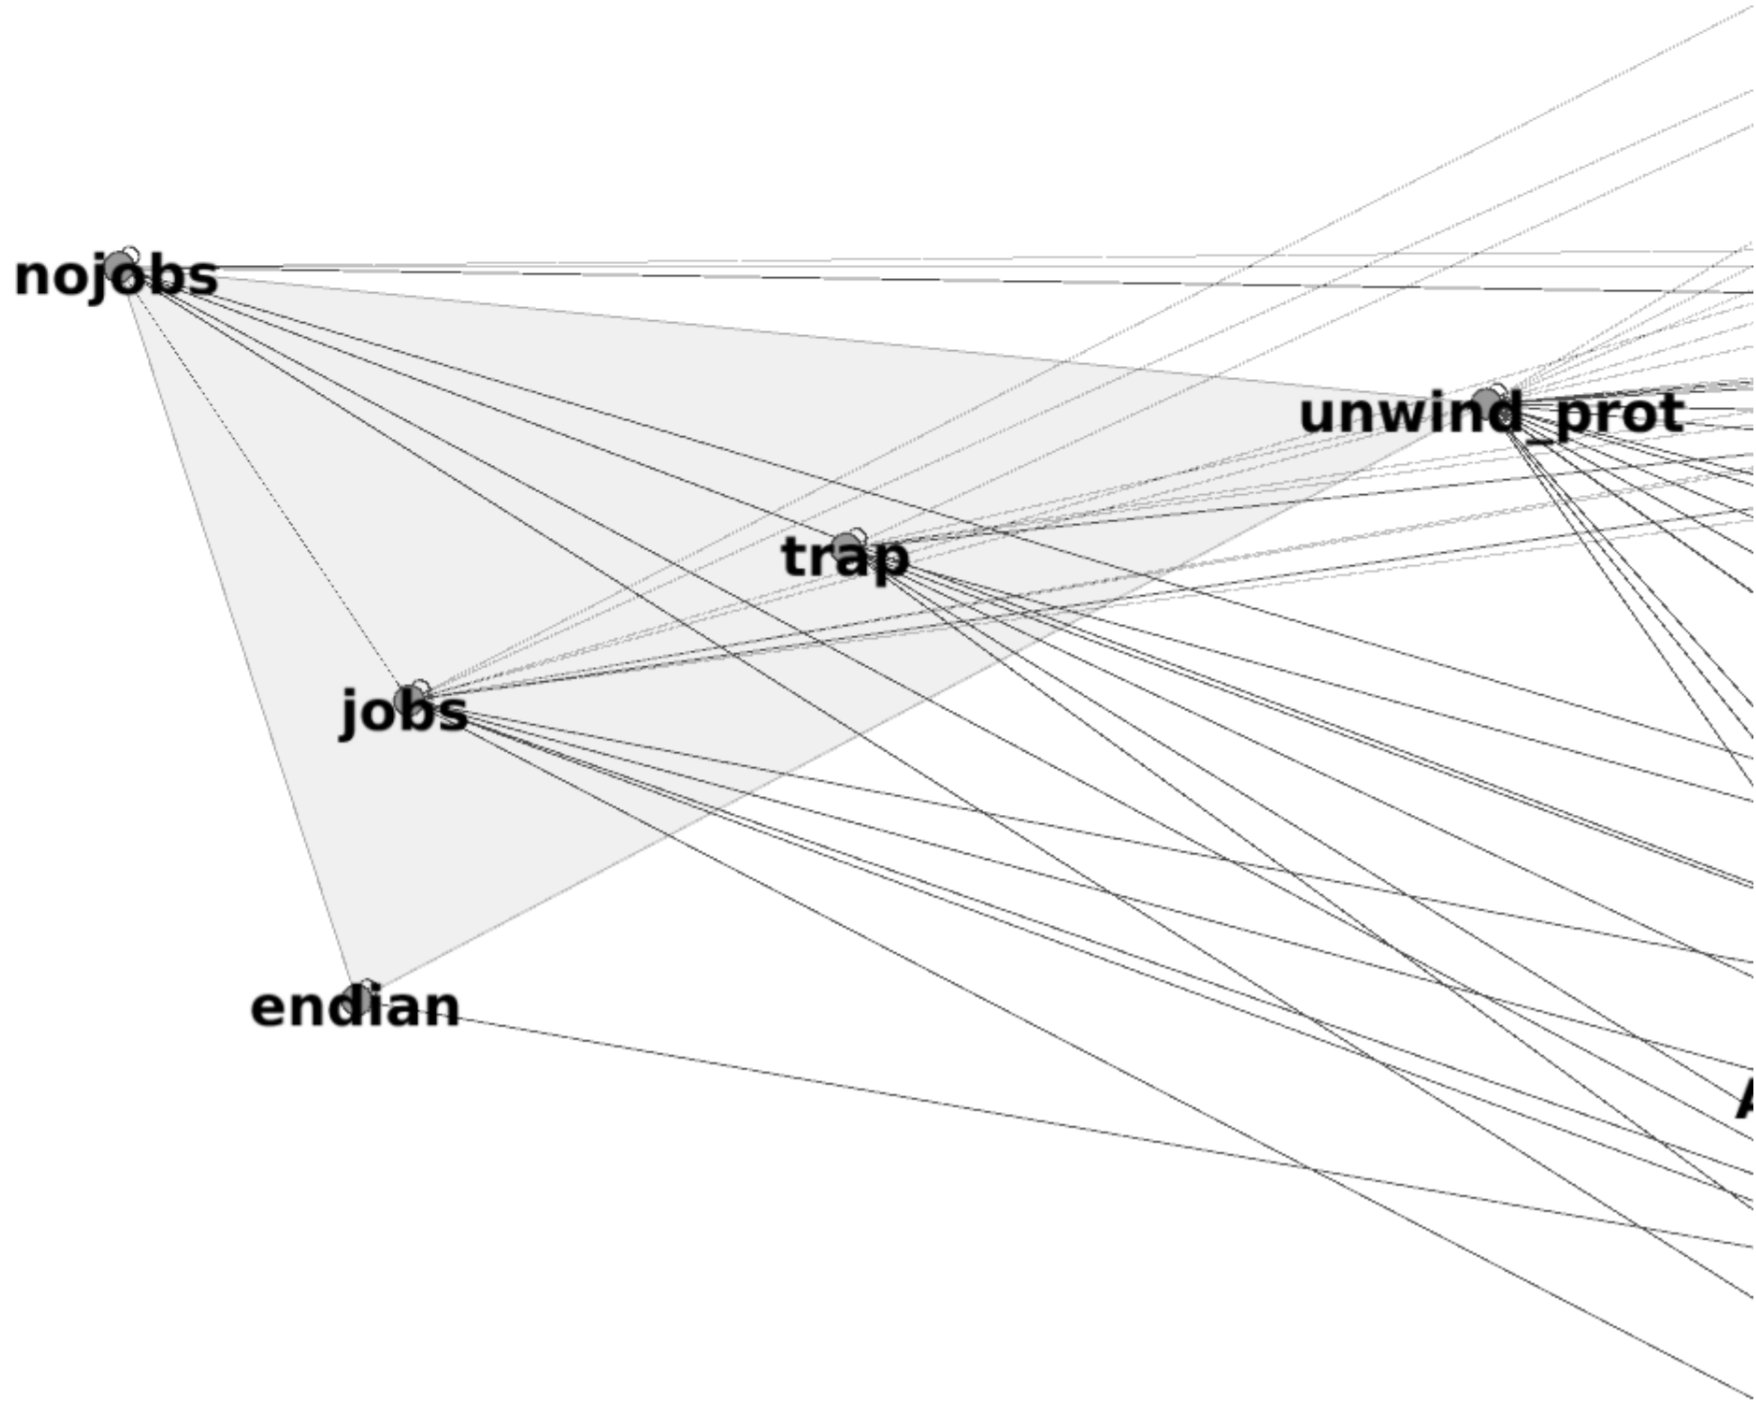
\includegraphics[width=0.7\textwidth]{bashJobControl.png}
		\end{center}
	\end{frame}

	\begin{frame}
		\frametitle{Commands}
		\begin{center}
			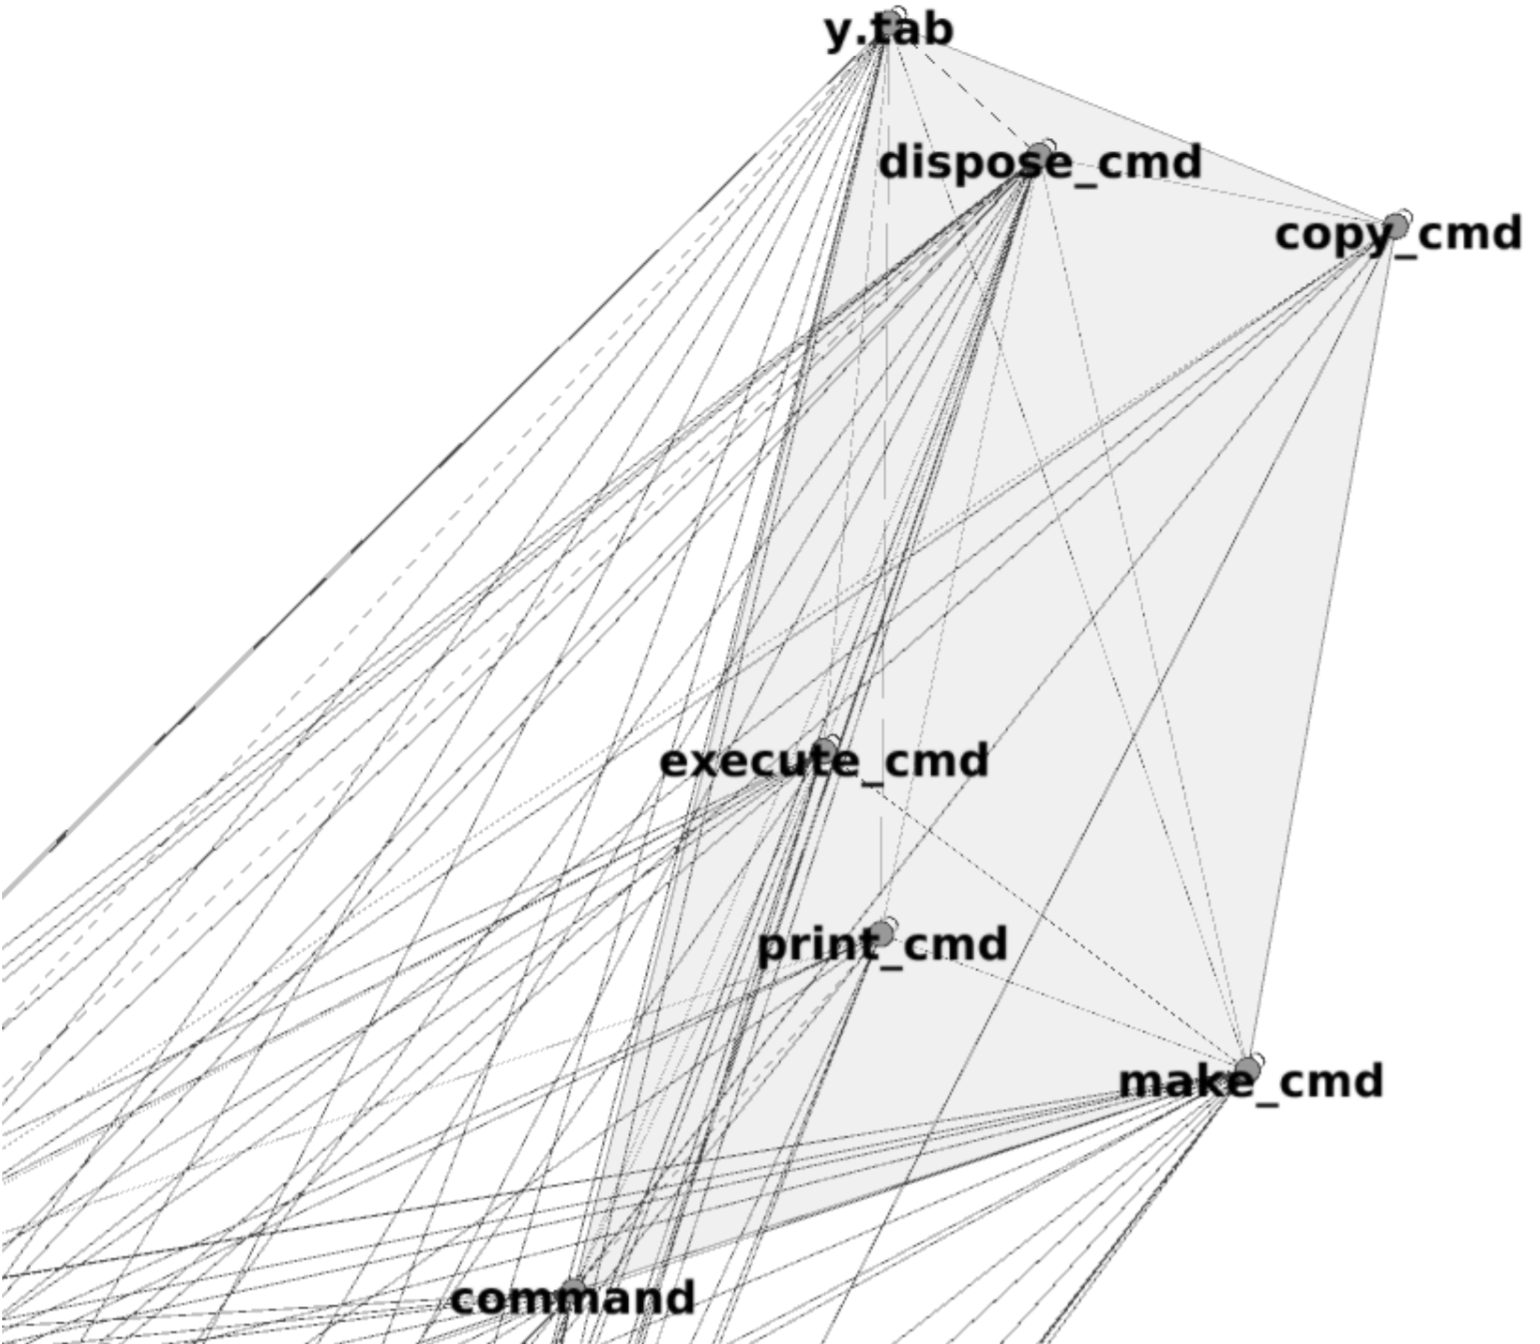
\includegraphics[width=0.7\textwidth]{bashCommands.png}
		\end{center}
	\end{frame}

	\section{Grep}

	\begin{frame}
		\frametitle{Grep}
		\framesubtitle{Следующая задача}
		Реализовать команду grep, 
		\begin{itemize}
			\item поддерживающую ключи
			\begin{itemize}
				\item \textit{-i} (нечувствительность к регистру)
				\item \textit{-w} (поиск только слов целиком)
				\item \textit{-A n} (распечатать n строк после строки с совпадением)
			\end{itemize}
			\item поддерживающую регулярные выражения в строке поиска
			\item использующую одну из библиотек для разбора аргументов командной строки
		\end{itemize}
	\end{frame}

	\begin{frame}[fragile]
		\frametitle{Примеры}
		\begin{minted}{bash}
> grep plugin build.gradle
    apply plugin: 'java'
    apply plugin: 'idea'
> cat build.gradle | grep plugin
    apply plugin: 'java'
    apply plugin: 'idea'
> grep -A 2 plugin build.gradle
    apply plugin: 'java'
    apply plugin: 'idea'
    group = 'ru.example'
    version = '1.0'
		\end{minted}
	\end{frame}

	\begin{frame}
		\frametitle{Замечания}
		\begin{itemize}
			\item Ожидается обоснование выбора библиотеки для работы с аргументами
			\begin{itemize}
				\item Какие библиотеки были рассмотрены
				\item Почему выбрана именно та, что выбрана
				\begin{itemize}
					\item кратко описать текстом
				\end{itemize}
			\end{itemize}
			\item Сдавать как новый пуллреквест из новой ветки на базе предыдущей
		\end{itemize}
	\end{frame}

\end{document}
